\documentclass[tikz]{standalone}

\usetikzlibrary{math}
\usetikzlibrary{backgrounds}
\usepackage{ifthen}

\begin{document}
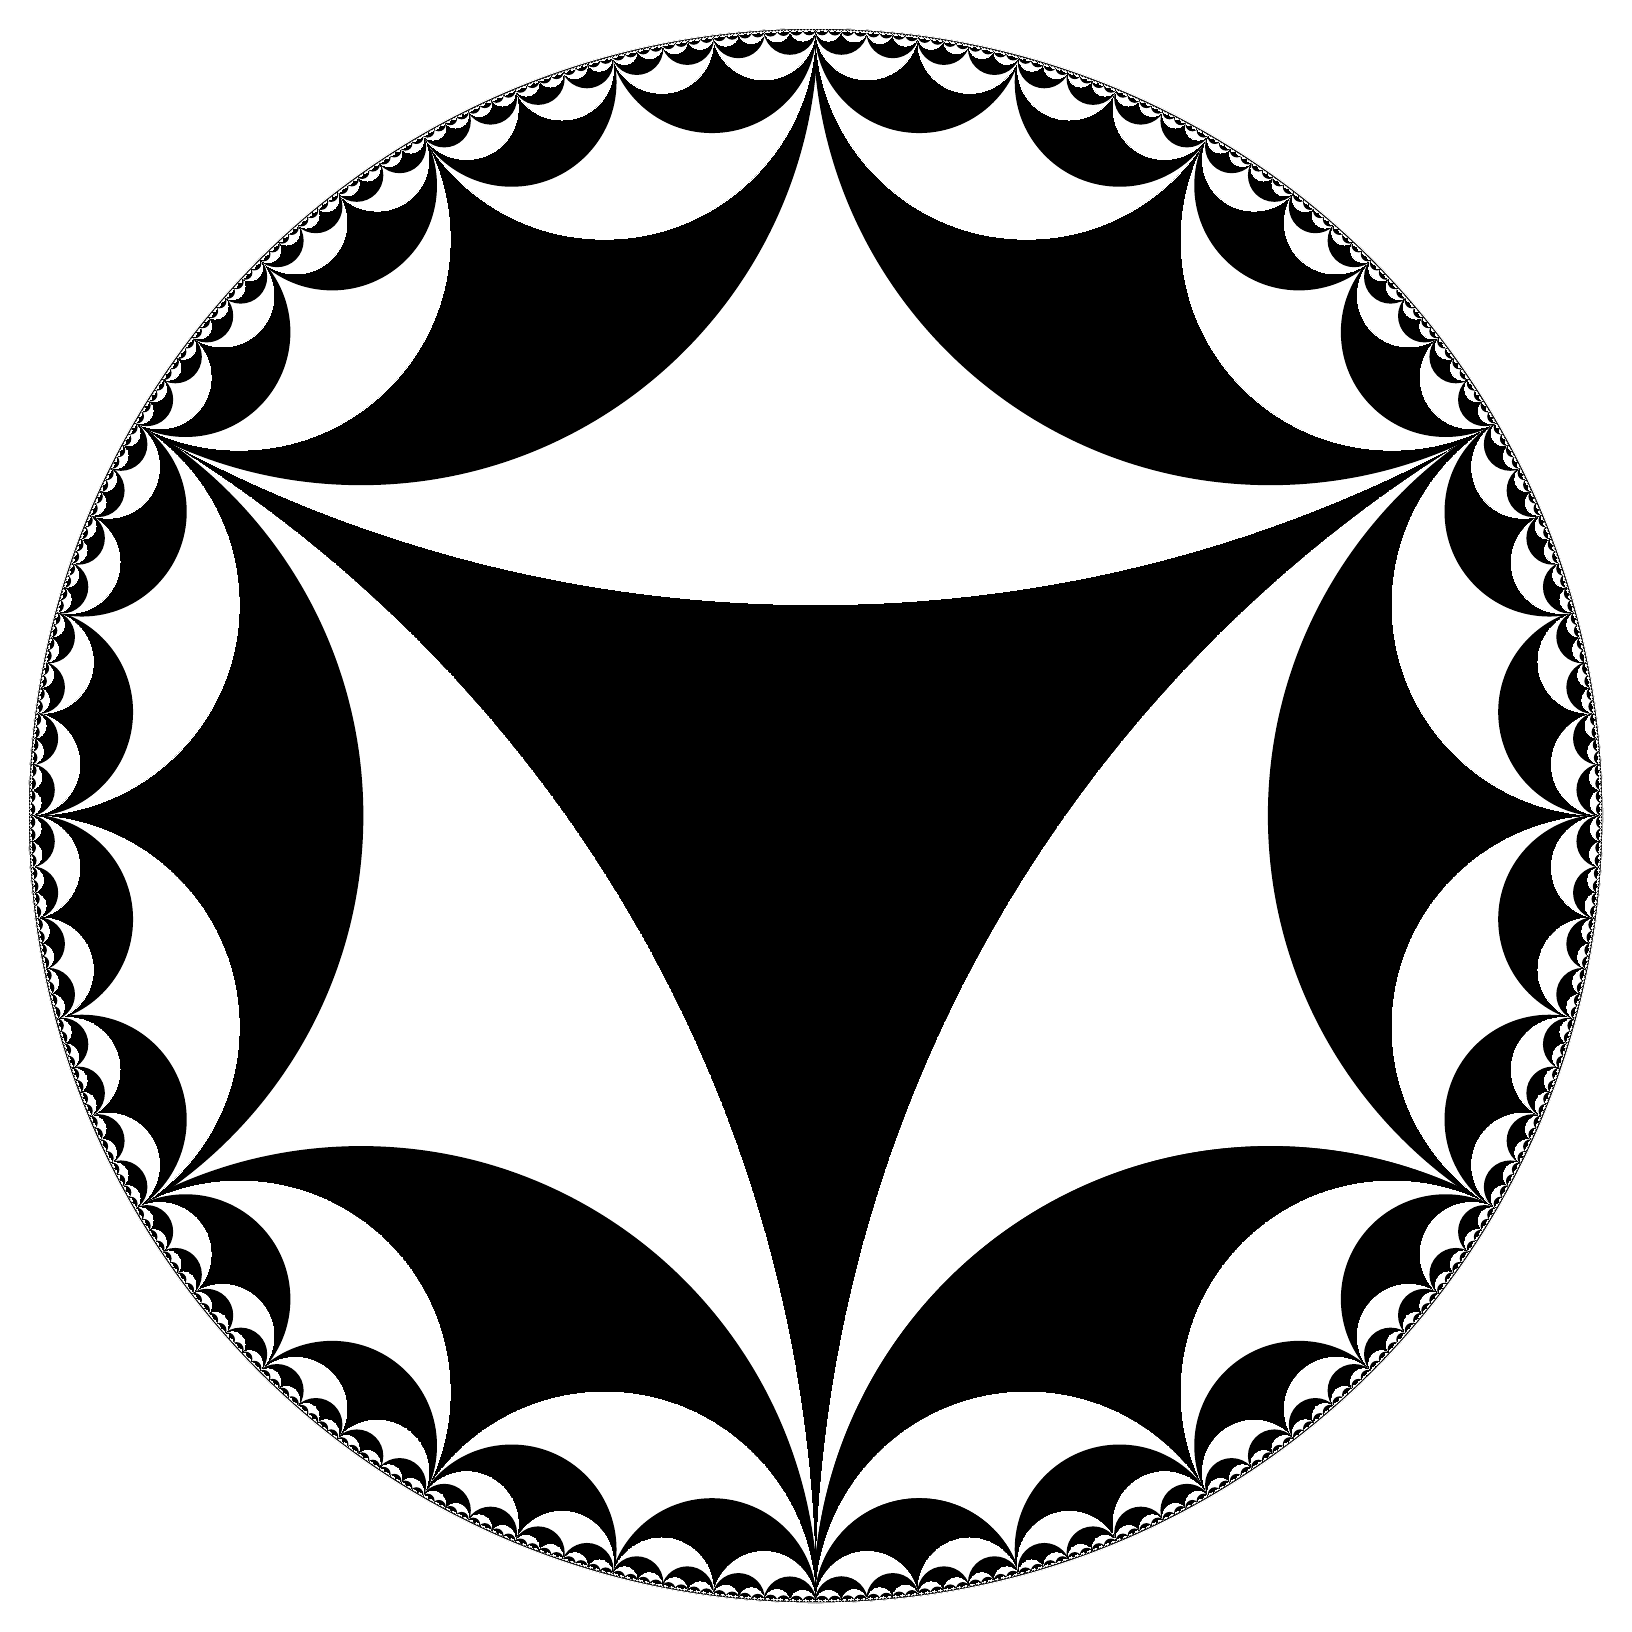
\begin{tikzpicture}
\fill [black] (0,0) circle (10);
    
\foreach \n in {0,...,9} {%
   \pgfmathsetmacro\x{3*2^\n}%
   \pgfmathsetmacro\alpha{360/\x}%
   \pgfmathsetmacro\radius{(sin(360/(\x*2))*10)/(cos(360/(\x*2)))}%
   \foreach \i in {0,1,...,\x} {%
      \pgfmathparse{sqrt(100+\radius*\radius)}\edef\radiusTwo{\pgfmathresult}%
      \pgfmathparse{\alpha*(\i+.5)-90}\edef\betai{\pgfmathresult}%
%
      \begin{scope}
      \clip (0,0) circle (10);
      \ifthenelse{\isodd{\n}}{
      	\fill[even odd rule,draw,black,line width=(2/(\n+1))*0.6mm] (\betai:\radiusTwo) circle (\radius);
      }
      {
      	\fill[even odd rule,draw,white,line width=0] (\betai:\radiusTwo) circle (\radius);
      }
      \end{scope}
   }
}
\draw [thin,white] (0,0) circle (10);
\end{tikzpicture}
\end{document}